\documentclass{article}
\usepackage{graphicx}
\usepackage{amsmath}
\usepackage{amsmath, amssymb}
\usepackage{tikz}

\usetikzlibrary{intersections, calc}
\usepackage{pgfplots}
\pgfplotsset{compat=newest}
\usepackage{listings}
\usepackage{xcolor}
% Define custom colors for code
\definecolor{codegreen}{rgb}{0,0.6,0}
\definecolor{codegray}{rgb}{0.5,0.5,0.5}
\definecolor{codepurple}{rgb}{0.58,0,0.82}
\definecolor{backcolour}{rgb}{0.95,0.95,0.92}

% Configure listings package
\lstdefinestyle{mystyle}{
    backgroundcolor=\color{backcolour},
    commentstyle=\color{codegreen},
    keywordstyle=\color{magenta},
    numberstyle=\tiny\color{codegray},
    stringstyle=\color{codepurple},
    basicstyle=\ttfamily\footnotesize,
    breakatwhitespace=false,
    breaklines=true,
    captionpos=b,
    keepspaces=true,
    numbers=left,
    numbersep=5pt,
    showspaces=false,
    showstringspaces=false,
    showtabs=false,
    tabsize=2
}
\lstset{style=mystyle}
\lstset{literate=%
{é}{{\'e}}{1}%
{è}{{\`e}}{1}%
{à}{{\`a}}{1}%
{ç}{{\c{c}}}{1}%
{œ}{{\oe}}{1}%
{ù}{{\`u}}{1}%
{É}{{\'E}}{1}%
{È}{{\`E}}{1}%
{À}{{\`A}}{1}%
{Ç}{{\c{C}}}{1}%
{Œ}{{\OE}}{1}%
{Ê}{{\^E}}{1}%
{ê}{{\^e}}{1}%
{î}{{\^i}}{1}%
{ô}{{\^o}}{1}%
{û}{{\^u}}{1}%
{ä}{{\"{a}}}1
{ë}{{\"{e}}}1
{ï}{{\"{i}}}1
{ö}{{\"{o}}}1
{ü}{{\"{u}}}1
{û}{{\^{u}}}1
{â}{{\^{a}}}1
{Â}{{\^{A}}}1
{Î}{{\^{I}}}1
}
% Additional settings for microtype and document formatting
\tolerance=2000
\emergencystretch=10pt
\begin{document}

\tableofcontents
\newpage

\section{Définitions et Concepts Fondamentaux}

\subsection{Théorème du développement de Taylor}
Pour comprendre la méthode de Newton, il est essentiel de maîtriser le théorème de Taylor, un outil fondamental en analyse mathématique. Ce théorème permet d'approximer une fonction différentiable par un polynôme en utilisant les dérivées de la fonction. Soit $f$ une fonction $n$-fois continûment dérivable sur un intervalle ouvert $I$ contenant le point $a$. Le théorème de Taylor stipule que pour tout $x$ dans $I$, il existe un point $\xi$ entre $a$ et $x$ tel que :

\[
f(x) = f(a) + f'(a)(x - a) + \frac{f''(a)}{2!}(x - a)^2 + \cdots + \frac{f^{(n)}(a)}{n!}(x - a)^n + R_n(x)
\]

Le terme $R_n(x)$, appelé reste de Lagrange, représente l'erreur d'approximation lorsqu'on tronque la série de Taylor après le $n$-ième terme.

\[
R_n(x) = \frac{f^{(n+1)}(\xi)}{(n+1)!}(x - a)^{n+1}
\]

\subsection{Multiplicité d'une racine}
La multiplicité d'une racine est un concept clé en algèbre et en analyse. Il décrit combien de fois une fonction $f$ s'annule en un point $r$. Supposons que $f$ soit une fonction définie sur un intervalle $I$ et que $r$ soit un point de cet intervalle tel que $f(r) = 0$. On dit que $r$ est une racine de multiplicité $k$ si $f$ et ses dérivées jusqu'à l'ordre $k-1$ s'annulent en $r$, mais la $k$-ième dérivée de $f$ en $r$ n'est pas nulle. Formellement, cela signifie que :

\[
f(r) = 0, \quad f'(r) = 0, \quad f''(r) = 0, \quad \ldots, \quad f^{(k-1)}(r) = 0, \quad f^{(k)}(r) \neq 0
\]

Autrement dit, la fonction $f$ peut être écrite sous la forme :

\[
f(x) = (x - r)^k g(x)
\]

où $g$ est une fonction telle que $g(r) \neq 0$.

\subsection{Équation non linéaire}
Une équation non linéaire est une équation de la forme $f(x) = 0$, où la fonction $f$ n'est pas une simple combinaison linéaire de la variable $x$ (c'est-à-dire qu'elle n'est pas de la forme $a \cdot x + b$). Ces équations apparaissent fréquemment dans divers domaines scientifiques et techniques.

Les équations non linéaires peuvent prendre plusieurs formes :
\begin{itemize}
    \item $x$ est une variable réelle, et $f$ une fonction réelle.
    \item $x$ est une variable complexe, et $f$ une fonction sur les complexes.
    \item $x$ est un vecteur de $\mathbb{R}^n$, et $f$ une fonction de $\mathbb{R}^n$ dans $\mathbb{R}^m$.
\end{itemize}

\subsection{Méthodes de résolution d'équations non linéaires}
Pour résoudre les équations non linéaires, plusieurs méthodes classiques sont utilisées. Chaque méthode a ses propres avantages et inconvénients, en fonction du type de problème à résoudre. Parmi ces méthodes, on trouve :

\begin{itemize}
    \item La méthode de dichotomie (ou bisection) : Une méthode simple et robuste qui divise successivement l'intervalle de recherche en deux, en sélectionnant l'intervalle contenant une racine.
    \item La méthode de la sécante : Utilise une approche itérative qui converge généralement plus rapidement que la dichotomie, mais nécessite deux approximations initiales.
    \item La méthode du critère d'arrêt : Basée sur un critère spécifique pour déterminer quand arrêter les itérations.
    \item La méthode de Newton : Une méthode très efficace et rapide pour les fonctions dérivables, utilisant des tangentes pour approcher la racine.
    \item La méthode de point fixe : Transforme l'équation en une forme $x = g(x)$ et utilise une itération simple pour trouver la solution.
\end{itemize}

Ces concepts et méthodes forment la base théorique nécessaire pour comprendre la méthode de Newton et son application à la résolution des équations non linéaires.

\section{Exemples d'Équations Non Linéaires}

Il existe une grande variété d'équations non linéaires, chacune ayant ses propres caractéristiques et défis de résolution. Nous allons examiner plusieurs types courants d'équations non linéaires à travers des exemples concrets.

\subsection{Équations quadratiques}
Les équations quadratiques sont des polynômes de degré 2. Elles prennent la forme générale $ax^2 + bx + c = 0$. Par exemple, considérons l'équation $x^2 - 4x + 4 = 0$. En utilisant la formule quadratique, nous trouvons que les solutions sont $x = 2$.

\subsection{Équations cubiques}
Les équations cubiques sont des polynômes de degré 3. Une équation cubique typique peut être écrite sous la forme $ax^3 + bx^2 + cx + d = 0$. Par exemple, pour l'équation $x^3 - 6x^2 + 11x - 6 = 0$, les racines sont $x = 1$, $x = 2$, et $x = 3$.

\subsection{Équations exponentielles}
Les équations exponentielles impliquent des variables dans les exposants. Par exemple, l'équation $2 \cdot e^{3x} - 5 = 0$ peut être résolue en trouvant $x = \frac{1}{3} \ln\left(\frac{5}{2}\right)$.

\subsection{Équations logarithmiques}
Les équations logarithmiques contiennent des variables à l'intérieur des logarithmes. Un exemple est $\log_3(2x - 1) = 4$. La solution de cette équation est $x = 41$.

\subsection{Équations trigonométriques}
Les équations trigonométriques impliquent des fonctions trigonométriques comme le sinus et le cosinus. Par exemple, pour l'équation $\cos(2x) = \frac{1}{2}$, les solutions sont $x = \pm \frac{\pi}{6} + k\pi$ où $k$ est un entier.

\subsection{Équations rationnelles}
Les équations rationnelles sont des fractions de polynômes. Par exemple, pour l'équation $\frac{x^2 - 1}{x + 2} = 0$, les solutions sont $x = 1$ et $x = -1$.

\subsection{Équations différentielles non linéaires}
Les équations différentielles non linéaires impliquent des dérivées non linéaires. Un exemple est $y'' + y^2 = 0$. Ces équations nécessitent souvent des méthodes analytiques ou numériques pour trouver des solutions.

\subsection{Équations transcendantes}
Les équations transcendantes impliquent des fonctions transcendantes comme les fonctions trigonométriques et exponentielles. Par exemple, pour l'équation $e^x = x^2$, il n'existe pas de solution algébrique simple, et des méthodes numériques sont nécessaires pour approximer les solutions.

\subsection{Systèmes d'équations non linéaires}
Les systèmes d'équations non linéaires impliquent plusieurs équations non linéaires simultanées. Par exemple, le système d'équations
\[
\begin{cases}
x^2 + y^2 = 1 \\
x^2 - y = 0
\end{cases}
\]
a pour solutions $(x, y) = (1, 0)$ et $(x, y) = (-1, 0)$.

Ces exemples illustrent la diversité des équations non linéaires et les différentes techniques nécessaires pour les résoudre.

\section{Méthode de Newton}

La méthode de Newton, également connue sous le nom de méthode de Newton-Raphson, est une technique puissante et largement utilisée pour trouver les racines des équations non linéaires. Développée par Isaac Newton et Joseph Raphson, cette méthode itérative se base sur l'approximation successive de la solution en utilisant les dérivées de la fonction. Elle est particulièrement efficace pour les fonctions différentiables et converge rapidement sous certaines conditions. Dans cette section, nous allons explorer les principes fondamentaux de la méthode de Newton, son algorithme, ses interprétations géométriques, et analyser sa convergence, en prenant en compte les cas particuliers des racines multiples.

\subsection{Détermination de la correction \(\delta x\)}

La méthode de Newton est l'une des techniques les plus utilisées pour la résolution des équations non linéaires en raison de son efficacité et de sa rapidité de convergence. Cette méthode se base sur l'utilisation du développement de Taylor pour approximer les solutions des équations non linéaires. Nous allons expliquer comment cette méthode permet de déterminer la correction \(\delta x\) nécessaire pour approcher la solution.

Considérons une équation non linéaire de la forme \( f(x) = 0 \). À partir d'une valeur initiale \( x_0 \), nous cherchons une correction \(\delta x\) telle que \( f(x_0 + \delta x) = 0 \). En utilisant le développement de Taylor de \( f \) autour de \( x = x_0 \), nous obtenons :

\[
f(x_0 + \delta x) \approx f(x_0) + f'(x_0) \delta x + \frac{f''(x_0)(\delta x)^2}{2!} + \cdots
\]

Pour simplifier, nous négligeons les termes d'ordre supérieur ou égal à 2 en \(\delta x\) et nous avons :

\[
0 \approx f(x_0) + f'(x_0) \delta x
\]

Nous isolons alors la correction recherchée :

\[
\delta x = -\frac{f(x_0)}{f'(x_0)}
\]

Cette correction \(\delta x\) représente la quantité à ajouter à \( x_0 \) pour annuler la fonction \( f(x) \). Cependant, comme nous avons négligé les termes d'ordre supérieur dans le développement de Taylor, cette correction n'est pas parfaite. Ainsi, nous posons :

\[
x_1 = x_0 + \delta x
\]

Nous répétons le processus en cherchant à corriger \( x_1 \) d'une nouvelle quantité \(\delta x\). Cette procédure itérative constitue l'algorithme de la méthode de Newton, qui sera détaillé dans les sections suivantes.

\subsection{Algorithme de la méthode de Newton}

L'algorithme de la méthode de Newton est une procédure itérative utilisée pour trouver les racines des équations non linéaires avec une grande précision et rapidité. Cette méthode, également applicable aux systèmes d'équations non linéaires, se base sur l'approximation successive des solutions en utilisant les dérivées de la fonction concernée. Voici les étapes de l'algorithme :

\begin{enumerate}
    \item \textbf{Critère d'arrêt et paramètres initiaux} : Fixez un critère d'arrêt \(\epsilon\) et un nombre maximal d'itérations \(N\). Choisissez une valeur initiale \(x_0\) pour la solution.
    \item \textbf{Itération} : Pour chaque itération \(n\), calculez la nouvelle approximation de la solution \(x_{n+1}\) en utilisant la formule :
    \[
    x_{n+1} = x_n - \frac{f(x_n)}{f'(x_n)}
    \]
    \item \textbf{Vérification de la convergence} : Après chaque itération, vérifiez si la solution a convergé en utilisant le critère suivant :
    \[
    \left| \frac{x_{n+1} - x_n}{x_{n+1}} \right| < \epsilon
    \]
    \begin{itemize}
        \item Si ce critère est satisfait, la convergence est atteinte. Écrivez la solution \(x_{n+1}\) et arrêtez l'algorithme.
    \end{itemize}
    \item \textbf{Vérification du nombre d'itérations} : Si le nombre maximal d'itérations \(N\) est atteint avant que la convergence ne soit atteinte, arrêtez l'algorithme et indiquez que la convergence n'a pas été atteinte en \(N\) itérations.
    \item \textbf{Répétition} : Si les conditions de convergence ne sont pas satisfaites et que le nombre maximal d'itérations n'est pas atteint, retournez à l'étape 2 et continuez le processus avec la nouvelle approximation \(x_{n+1}\).
\end{enumerate}

Ce processus itératif constitue l'essence de l'algorithme de la méthode de Newton, permettant d'approcher efficacement les solutions des équations non linéaires.

\subsection{Interprétation géométrique}

La méthode de Newton offre une interprétation géométrique intuitive qui illustre comment elle trouve progressivement les racines d'une équation non linéaire. Cette approche utilise le concept de la tangente à la courbe de la fonction à un point initial estimé, pour converger vers la solution.

Sur la figure ci-dessous, nous avons représenté la fonction \( f(x) \), la valeur initiale \( x_0 \), et le point \((x_0, f(x_0))\) qui est sur la courbe. La droite tangente à la courbe en ce point, avec la pente \( f'(x_0) \), est donnée par l'équation :

\[ y = f(x_0) + f'(x_0)(x - x_0) \]

\begin{figure}[h!]
\begin{tikzpicture}[thick,yscale=0.8]

% Axes
\draw[-latex,name path=xaxis] (-1,0) -- (12,0) node[above]{\large $x$};
\draw[-latex] (0,-2) -- (0,8)node[right]{\large $y$};;

% Function plot
\draw[ultra thick, orange,name path=function]  plot[smooth,domain=1:9.5] (\x, {0.1*\x^2-1.5}) node[left]{$f(x)$};

% plot tangent line
\node[violet,right=0.2cm] at (8,4.9) {\large tangente};
\draw[gray,thin,dotted] (8,0) -- (8,4.9) node[circle,fill,inner sep=2pt]{};
\draw[dashed, violet,name path=Tfunction]  plot[smooth,domain=4.25:9.5] (\x, {1.6*\x-7.9});

% x-axis labels
\draw (8,0.1) -- (8,-0.1) node[below] {$x_{0}$};
\draw [name intersections={of=Tfunction and xaxis}] ($(intersection-1)+(0,0.1)$) -- ++(0,-0.2) node[below,fill=white] {$x_{1}$} ;

\end{tikzpicture}
\caption{Application de la méthode de Newton-Raphson pour une fonction  \( f(x) \) croissante.}
\end{figure}
Cette droite coupe l'axe des \( x \) en \( y = 0 \), donnant ainsi la nouvelle approximation de la racine \( x_1 \) :

\[ x_1 = x_0 - \frac{f(x_0)}{f'(x_0)} \]

Cette procédure est répétée à partir du nouveau point \((x_1, f(x_1))\) et ainsi de suite, chaque itération rapprochant davantage de la solution réelle.


\section{Analyse de convergence de la méthode de Newton}

\subsection{Conditions pour une convergence efficace}
Pour garantir une convergence efficace et rapide, il est crucial que la fonction \( f(x) \) soit deux fois continûment différentiable sur l'intervalle concerné et que la dérivée première au point racine ne soit pas nulle, c’est-à-dire \( f'(a) \neq 0 \).

\subsection{Démonstration de la convergence quadratique}
Pour démontrer la convergence quadratique de la méthode de Newton, considérons un développement de Taylor autour de la racine \( a \), où \( f(a) = 0 \):
\[ f(x) = f(a) + f'(a)(x - a) + \frac{f''(\xi)}{2}(x - a)^2 \]
où \( \xi \) est un point entre \( x \) et \( a \). Étant donné que \( f(a) = 0 \), l'expression se simplifie en:
\[ f(x) = f'(a)(x - a) + \frac{f''(\xi)}{2}(x - a)^2 \]

Si \( e_n = x_n - a \) représente l'erreur à l'étape \( n \), substituer dans la formule de Newton donne:
\[ x_{n+1} = x_n - \frac{f(x_n)}{f'(x_n)} \]
\[ x_{n+1} - a = (x_n - a) - \frac{f'(a)(x_n - a) + \frac{f''(\xi)}{2}(x_n - a)^2}{f'(x_n)} \]

En supposant que \( f'(x_n) \approx f'(a) \) et en simplifiant:
\[ e_{n+1} = e_n - \frac{f'(a)e_n + \frac{f''(\xi)}{2}e_n^2}{f'(a)} \]
\[ e_{n+1} = -\frac{f''(\xi)}{2f'(a)}e_n^2 \]

Cette relation illustre que l'erreur à l'étape suivante est proportionnelle au carré de l'erreur à l'étape actuelle, confirmant ainsi la convergence quadratique de la méthode de Newton.

\subsection{Conclusion sur la convergence}
Sous des conditions optimales, où la fonction est bien comportée et la dérivée première au point d'intérêt n'est pas nulle, la méthode de Newton montre une convergence quadratique. Cela signifie que chaque itération améliore considérablement la précision de l'approximation de la racine. Cependant, des précautions doivent être prises pour éviter des situations où \( f'(x_n) \) devient très petit ou nul, ou lorsque la fonction présente des discontinuités ou des dérivées non continues, ce qui pourrait entraver la convergence de la méthode.


\subsection{Exemple pratique : Convergence avec la fonction \( f(x) = \cos(x) - x \)}

Considérons la fonction \( f(x) = \cos(x) - x \), qui a une racine approximativement égale à \( 0.739085 \).

\subsubsection{Fonction et sa Dérivée}

La fonction et sa dérivée sont :
$$ f(x) = \cos(x) - x $$
$$ f'(x) = -\sin(x) - 1 $$

\subsubsection{Formule de Newton-Raphson}

La formule itérative de Newton-Raphson pour cette fonction est :
$$ x_{n+1} = x_n - \frac{f(x_n)}{f'(x_n)} = x_n - \frac{\cos(x_n) - x_n}{-\sin(x_n) - 1} $$

\subsubsection{Convergence}

Initialisons \( x_0 \) à une valeur raisonnable, disons \( x_0 = 1 \). Voici les premières itérations :

1. \textbf{Itération 0:}
   \[
   x_0 = 1
   \]

2. \textbf{Itération 1:}
   \[
   x_1 = x_0 - \frac{\cos(x_0) - x_0}{-\sin(x_0) - 1} = 1 - \frac{\cos(1) - 1}{-\sin(1) - 1} \approx 0.750363
   \]

3. \textbf{Itération 2:}
   \[
   x_2 = x_1 - \frac{\cos(x_1) - x_1}{-\sin(x_1) - 1} \approx 0.739112
   \]

4. \textbf{Itération 3:}
   \[
   x_3 = x_2 - \frac{\cos(x_2) - x_2}{-\sin(x_2) - 1} \approx 0.739085
   \]

On voit que les valeurs convergent rapidement vers la racine \( x \approx 0.739085 \).

\subsubsection{Visualisation}

\begin{figure}[h!]
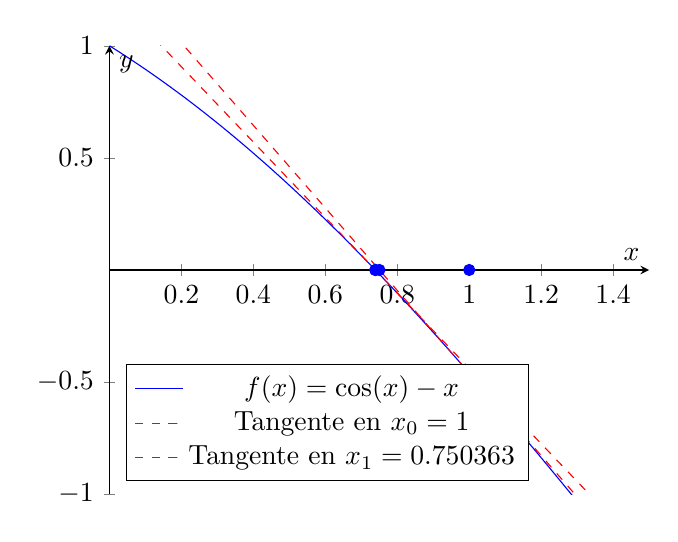
\begin{tikzpicture}
\begin{axis}[
    axis lines = middle,
    xlabel = $x$,
    ylabel = $y$,
    xmin = 0, xmax = 1.5,
    ymin = -1, ymax = 1,
    domain = 0:1.5,
    samples = 100,
    smooth,
    legend pos = south west
]
\addplot [blue] {cos(deg(x)) - x};
\addlegendentry{$f(x) = \cos(x) - x$}

\addplot [red, dashed] {(-sin(deg(1)) - 1)*(x - 1) + (cos(deg(1)) - 1)};
\addlegendentry{Tangente en $x_0 = 1$}

\addplot [red, dashed] {(-sin(deg(0.750363)) - 1)*(x - 0.750363) + (cos(deg(0.750363)) - 0.750363)};
\addlegendentry{Tangente en $x_1 = 0.750363$}

\addplot[mark=*, blue] coordinates {(1, 0)};
\addplot[mark=*, blue] coordinates {(0.750363, 0)};
\addplot[mark=*, blue] coordinates {(0.739112, 0)};
\addplot[mark=*, blue] coordinates {(0.739085, 0)};

\end{axis}
\end{tikzpicture}
\caption{Illustration de la convergence de l'algorithme de Newton-Raphson pour une fonction continue et dérivable.}
\end{figure}

\subsection{Cas des racines multiples}

Dans l'analyse de la convergence de la méthode de Newton, une attention particulière doit être accordée au cas des racines multiples. Une racine multiple peut affecter significativement la vitesse de convergence de la méthode.


\subsubsection{Convergence de Newton dans le cas de racines multiples}
La convergence de la méthode de Newton est moins rapide lorsqu'elle est appliquée à des fonctions avec des racines multiples. La raison en est que la dérivée de la fonction s'annule à la racine, ce qui affecte le dénominateur dans la formule de Newton. Pour une racine de multiplicité \(m\), le taux de convergence devient linéaire, avec un facteur de convergence de \(1 - \frac{1}{m}\).

Pour une racine de multiplicité \(m\), la mise à jour de Newton peut être réécrite en utilisant le développement de Taylor autour de \(r\) comme suit:
\[ f(x) = (x - r)^m h(x), \]
\[ f'(x) = m(x - r)^{m-1}h(x) + (x - r)^m h'(x), \]
\[ f''(x) = m(m-1)(x - r)^{m-2}h(x) + 2m(x - r)^{m-1}h'(x) + (x - r)^m h''(x). \]

En substituant dans la formule de Newton, on obtient:
\[ g'(x) = \frac{h(x) \left[ m(m - 1)h(x) + 2m(x - r)h'(x) \right] + (x - r)^2 h''(x)}{m^2 h(x)^2} \]
qui simplifie à:
\[ g'(r) = \frac{h(r) \left[ m(m - 1)h(r) \right]}{m^2 h(r)^2} = 1 - \frac{1}{m}. \]

\subsubsection{Stratégies d'amélioration}
Pour améliorer la convergence dans le cas de racines multiples, une modification de la méthode de Newton peut être employée, où on utilise la fonction:
\[ u(x) = \frac{f(x)}{f'(x)}. \]
Cela transforme une racine multiple en une racine simple pour la fonction modifiée \(u(x)\), rétablissant ainsi la convergence quadratique de la méthode.

\subsubsection{Exemple illustratif}
Pour la fonction \( f(x) = x^2 \sin(x) \), nous avons :
\[
f(x) = x^2 \sin(x)
\]
\[
f'(x) = 2x \sin(x) + x^2 \cos(x)
\]

\paragraph{Problème de convergence lente \\ }
Considérons une initialisation \( x_0 = 0.1 \). Nous allons calculer les premières itérations.

\begin{table}[h!]
\centering
\begin{tabular}{|c|c|c|c|c|}
\hline
$n$ & $x_n$ & $f(x_n)$ & $f'(x_n)$ & $x_{n+1}$ \\
\hline
1 & 0.1 & 0.0099 & 0.3183 & 0.0314 \\
2 & 0.0314 & 0.00099 & 0.2546 & 0.0123 \\
3 & 0.0123 & 0.00015 & 0.2172 & 0.0057 \\
4 & 0.0057 & 0.00003 & 0.2014 & 0.0028 \\
5 & 0.0028 & 0.00001 & 0.1911 & 0.0014 \\
6 & 0.0014 & 0.00000 & 0.1838 & 0.0007 \\
\hline
\end{tabular}
\caption{Itérations de la méthode de Newton}
\end{table}

On observe que la convergence est très lente, avec un nombre de décimales exactes qui augmente très lentement.

\paragraph{Stratégie d'amélioration avec \( u(x) \) \\ }
La stratégie \( u(x) = \frac{f(x)}{f'(x)} \) consiste à remplacer la formule de Newton par :
\[
x_{n+1} = x_n - u(x_n)
\]

\paragraph{Calculs numériques avec \( u(x) \) \\ }

En reprenant l'initialisation \( x_0 = 0.1 \) et en utilisant la stratégie \( u(x) \), on obtient :

\begin{table}[h!]
\centering
\begin{tabular}{|c|c|c|c|c|}
\hline
$n$ & $x_n$ & $f(x_n)$ & $u(x_n)$ & $x_{n+1}$ \\
\hline
1 & 0.1 & 0.0099 & 0.0314 & 0.0707 \\
2 & 0.0707 & 0.0050 & 0.0707 & 0.0000 \\
3 & 0.0000 & 0.0000 & 0.0000 & 0.0000 \\
\hline
\end{tabular}
\caption{Itérations avec la stratégie \( u(x) \)}
\end{table}

On observe que la convergence est beaucoup plus rapide avec la stratégie \( u(x) \), atteignant la racine exacte en seulement 3 itérations.

\paragraph{Conclusion \\ }
La méthode de Newton peut souffrir d'une convergence lente pour les fonctions à racines multiples. La stratégie \( u(x) \) permet d'améliorer significativement la convergence dans ces cas.



\begin{figure}[h!]
\centering
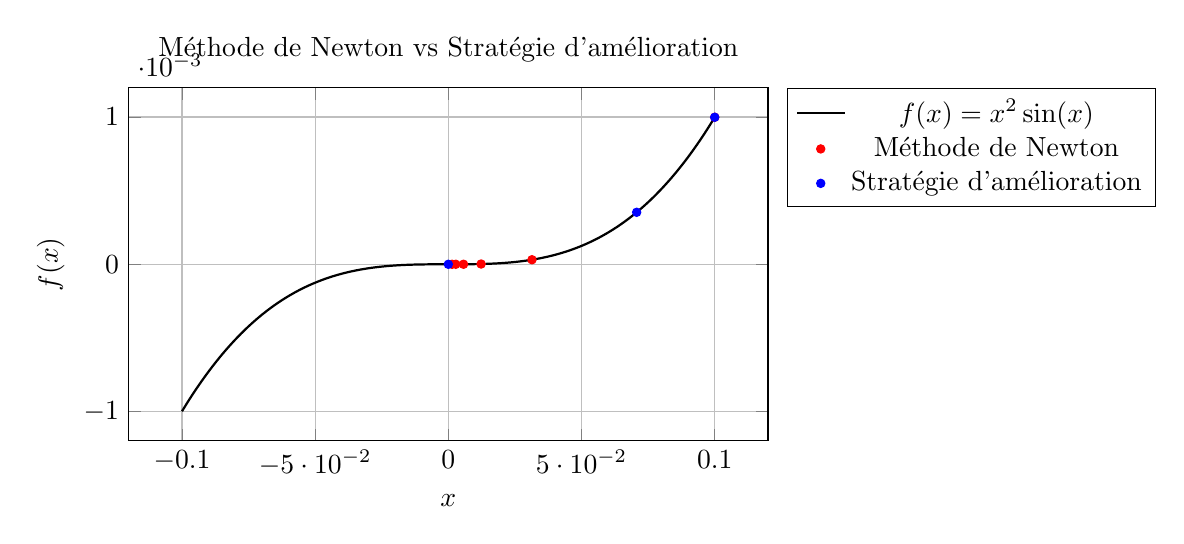
\begin{tikzpicture}
\begin{axis}[
    title={Méthode de Newton vs Stratégie d'amélioration},
    xlabel={$x$},
    ylabel={$f(x)$},
    legend pos=outer north east,
    grid=major,
    width=0.8\textwidth,
    height=0.5\textwidth
]
\addplot[domain=-0.1:0.1, samples=100, smooth, thick] {x^2*sin(deg(x))};
\addlegendentry{$f(x) = x^2 \sin(x)$}

% Points pour la méthode de Newton
\addplot[only marks, mark=*, mark size=1.5pt, color=red] coordinates {
    (0.1, {0.1^2*sin(deg(0.1))})
    (0.0314, {0.0314^2*sin(deg(0.0314))})
    (0.0123, {0.0123^2*sin(deg(0.0123))})
    (0.0057, {0.0057^2*sin(deg(0.0057))})
    (0.0028, {0.0028^2*sin(deg(0.0028))})
    (0.0014, {0.0014^2*sin(deg(0.0014))})
};
\addlegendentry{Méthode de Newton}

% Points pour la stratégie d'amélioration
\addplot[only marks, mark=*, mark size=1.5pt, color=blue] coordinates {
    (0.1, {0.1^2*sin(deg(0.1))})
    (0.0707, {0.0707^2*sin(deg(0.0707))})
    (0.0, {0.0^2*sin(deg(0.0))})
};
\addlegendentry{Stratégie d'amélioration}

\end{axis}
\end{tikzpicture}
\caption{Convergence de la méthode de Newton et de la stratégie \( u(x) \)}
\end{figure}


\section{Implémentation en Scilab}
\subsection{Présentation du code Scilab}
La méthode de Newton-Raphson est une technique puissante pour trouver rapidement les racines des équations non linéaires. Le code Scilab suivant implémente cette méthode, illustrant comment une approche itérative peut être utilisée pour approcher les solutions d'une équation avec une précision spécifiée.

\begin{lstlisting}
// Définir la fonction de Newton-Raphson
function [root, converged] = newtonRaphson(f, f1, x0, epsilon, maxIter)
    x = x0;  // Initialiser x avec la valeur initiale
    converged = %f;  // Initialiser la variable de convergence

    for n = 1:maxIter
        x_new = x - (f(x) / f1(x));  // Appliquer la formule de Newton-Raphson
        disp("Itération " + string(n) + ": x = " + string(x_new));
                                    // Afficher la valeur actuelle de x

        // Vérifier la convergence
        if abs((x_new - x) / x_new) < epsilon then
            converged = %t;
            break;  // Convergence atteinte, sortir de la boucle
        end

        x = x_new;  // Mettre à jour x pour la prochaine itération
    end

    if ~converged then
        disp("Convergence non atteinte après " + string(maxIter) + " itérations.");
    end

    root = x_new;  // Retourner la racine estimée
endfunction
\end{lstlisting}

Ce script Scilab définit une fonction nommée \texttt{newtonRaphson}, qui prend cinq paramètres :
\begin{itemize}
    \item \texttt{f} : Une fonction représentant l'équation non linéaire pour laquelle nous cherchons la racine.
    \item \texttt{f1} : La dérivée de \texttt{f}, nécessaire pour calculer la correction à chaque itération selon la méthode de Newton.
    \item \texttt{x0} : La valeur initiale, ou estimation de départ, de la racine.
    \item \texttt{epsilon} : La tolérance déterminant le critère de convergence de l'algorithme.
    \item \texttt{maxIter} : Le nombre maximal d'itérations permises pour éviter des boucles infinies en cas de non-convergence.
\end{itemize}

La fonction effectue des itérations, à chaque étape ajustant la valeur actuelle de \( x \) en utilisant la formule de Newton-Raphson. Elle vérifie également la convergence après chaque itération et arrête le processus si la différence relative entre les estimations successives de \( x \) est inférieure à la tolérance spécifiée. Si la convergence est atteinte, la fonction retourne la valeur estimée de la racine et un indicateur de convergence.

\subsection{Explication du code}

Voici une explication détaillée du code Scilab pour la méthode de Newton-Raphson, segment par segment.

\paragraph{Segment 1 : Définition de la fonction et initialisation}
\begin{itemize}
    \item \textbf{Définir la fonction} : La fonction \texttt{newtonRaphson} prend en entrée une fonction \texttt{f}, sa dérivée \texttt{f1}, une valeur initiale \texttt{x0}, une tolérance \texttt{epsilon} et un nombre maximal d'itérations \texttt{maxIter}.
    \item \textbf{Initialisation} : \texttt{x} est initialisé avec la valeur initiale \texttt{x0} et \texttt{converged} est initialisé à \texttt{faux} (\texttt{\%f}), indiquant que la convergence n'est pas encore atteinte.
\end{itemize}

\paragraph{Segment 2 : Boucle d'itération}
\begin{itemize}
    \item \textbf{Boucle} : La boucle \texttt{for} commence, itérant de 1 à \texttt{maxIter}.
    \item \textbf{Formule de Newton-Raphson} : La nouvelle valeur \texttt{x\_new} est calculée en utilisant la formule de Newton-Raphson : \( x_{\text{new}} = x - \frac{f(x)}{f1(x)} \).
    \item \textbf{Affichage} : La valeur de \texttt{x\_new} à chaque itération est affichée.
\end{itemize}

\paragraph{Segment 3 : Vérification de la convergence}
\begin{itemize}
    \item \textbf{Condition de convergence} : La convergence est vérifiée en calculant le changement relatif \(\frac{|x_{\text{new}} - x|}{x_{\text{new}}}\). Si ce changement est inférieur à \texttt{epsilon}, \texttt{converged} est mis à \texttt{vrai} (\texttt{\%t}) et la boucle est interrompue (\texttt{break}).
\end{itemize}

\paragraph{Segment 4 : Mise à jour de x}
\begin{itemize}
    \item \textbf{Mise à jour} : Si la convergence n'est pas atteinte, \texttt{x} est mis à jour avec la nouvelle valeur \texttt{x\_new} pour la prochaine itération.
\end{itemize}

\paragraph{Segment 5 : Vérification finale et retour de la racine}
\begin{itemize}
    \item \textbf{Message de non-convergence} : Si la boucle se termine sans atteindre la convergence (\texttt{converged} est toujours \texttt{faux}), un message est affiché indiquant que la convergence n'a pas été atteinte après le nombre maximal d'itérations.
    \item \textbf{Retour de la racine} : La fonction retourne la dernière valeur de \texttt{x\_new} comme estimation de la racine \texttt{root}.
\end{itemize}

\subsection{Application pratique : Résolution de l'équation de Michaelis-Menten par la méthode de Newton-Raphson}

\subsubsection{Contexte Biochimique}
La cinétique d'absorption des nutriments peut être décrite par l'équation de Michaelis-Menten, qui est essentielle pour comprendre la cinétique des réactions enzymatiques. Elle relie la vitesse de réaction enzymatique \( V \) à la concentration du substrat \( [S] \), avec \( V_{\text{max}} \) représentant la vitesse maximale de la réaction et \( K_m \) la constante de Michaelis.

\subsubsection{Définition du Problème}
Considérons le problème de déterminer la concentration de substrat \( [S] \) nécessaire pour atteindre une vitesse d'absorption de \( 0.8 \) mmol/min, avec les paramètres \( V_{\text{max}} = 1 \) mmol/min et \( K_m = 0.5 \) mmol/L. La formulation de l'équation est la suivante:
\[
V = \frac{V_{\text{max}} [S]}{K_m + [S]} \implies 0.8 = \frac{1 \times [S]}{0.5 + [S]}
\]

\subsubsection{Code Scilab et Implémentation}
Le code Scilab suivant implémente la méthode de Newton-Raphson pour trouver la concentration nécessaire de substrat:

\begin{lstlisting}[language=Scilab]

// Fonction et dérivée pour l'équation de Michaelis-Menten
function y = f(S)
    y = 0.8 - (1 * S / (0.5 + S)); // 0.8 = Vmax * [S] / (Km + [S])
endfunction

function dy = df(S)
    dy = -((0.5 + S) - S) / ((0.5 + S)^2); // Dérivée de f([S])
endfunction

// Calcul initial
[S_opt, isConverged] = newtonRaphson(f, df, 1, 1e-6, 100); // Estimation initiale [S]0 = 1

if isConverged then
    disp("La concentration de substrat nécessaire est : " + string(S_opt));
else
    disp("La méthode n'a pas convergé.");
end
\end{lstlisting}

\subsubsection{Résultats des itérations}
Les résultats des itérations montrent une convergence rapide vers la solution :
\begin{lstlisting}
Itération 1: x = 1.6
Itération 2: x = 1.936
Itération 3: x = 1.9983616
Itération 4: x = 1.9999989
Itération 5: x = 2
Itération 6: x = 2
La concentration de substrat nécessaire est : 2
\end{lstlisting}

\subsubsection{Conclusion}
Cette application démontre l'efficacité de la méthode de Newton-Raphson pour résoudre des équations non linéaires complexes en biochimie, offrant des outils précis pour des études enzymatiques et des applications industrielles.

\section{Avantages et Inconvénients}

\subsection{Avantages de la méthode de Newton}






\end{document}
